\documentclass[twoside]{book}

% Packages required by doxygen
\usepackage{fixltx2e}
\usepackage{calc}
\usepackage{doxygen}
\usepackage[export]{adjustbox} % also loads graphicx
\usepackage{graphicx}
\usepackage[utf8]{inputenc}
\usepackage{makeidx}
\usepackage{multicol}
\usepackage{multirow}
\PassOptionsToPackage{warn}{textcomp}
\usepackage{textcomp}
\usepackage[nointegrals]{wasysym}
\usepackage[table]{xcolor}

% Font selection
\usepackage[T1]{fontenc}
\usepackage[scaled=.90]{helvet}
\usepackage{courier}
\usepackage{amssymb}
\usepackage{sectsty}
\renewcommand{\familydefault}{\sfdefault}
\allsectionsfont{%
  \fontseries{bc}\selectfont%
  \color{darkgray}%
}
\renewcommand{\DoxyLabelFont}{%
  \fontseries{bc}\selectfont%
  \color{darkgray}%
}
\newcommand{\+}{\discretionary{\mbox{\scriptsize$\hookleftarrow$}}{}{}}

% Page & text layout
\usepackage{geometry}
\geometry{%
  a4paper,%
  top=2.5cm,%
  bottom=2.5cm,%
  left=2.5cm,%
  right=2.5cm%
}
\tolerance=750
\hfuzz=15pt
\hbadness=750
\setlength{\emergencystretch}{15pt}
\setlength{\parindent}{0cm}
\setlength{\parskip}{3ex plus 2ex minus 2ex}
\makeatletter
\renewcommand{\paragraph}{%
  \@startsection{paragraph}{4}{0ex}{-1.0ex}{1.0ex}{%
    \normalfont\normalsize\bfseries\SS@parafont%
  }%
}
\renewcommand{\subparagraph}{%
  \@startsection{subparagraph}{5}{0ex}{-1.0ex}{1.0ex}{%
    \normalfont\normalsize\bfseries\SS@subparafont%
  }%
}
\makeatother

% Headers & footers
\usepackage{fancyhdr}
\pagestyle{fancyplain}
\fancyhead[LE]{\fancyplain{}{\bfseries\thepage}}
\fancyhead[CE]{\fancyplain{}{}}
\fancyhead[RE]{\fancyplain{}{\bfseries\leftmark}}
\fancyhead[LO]{\fancyplain{}{\bfseries\rightmark}}
\fancyhead[CO]{\fancyplain{}{}}
\fancyhead[RO]{\fancyplain{}{\bfseries\thepage}}
\fancyfoot[LE]{\fancyplain{}{}}
\fancyfoot[CE]{\fancyplain{}{}}
\fancyfoot[RE]{\fancyplain{}{\bfseries\scriptsize Generated by Doxygen }}
\fancyfoot[LO]{\fancyplain{}{\bfseries\scriptsize Generated by Doxygen }}
\fancyfoot[CO]{\fancyplain{}{}}
\fancyfoot[RO]{\fancyplain{}{}}
\renewcommand{\footrulewidth}{0.4pt}
\renewcommand{\chaptermark}[1]{%
  \markboth{#1}{}%
}
\renewcommand{\sectionmark}[1]{%
  \markright{\thesection\ #1}%
}

% Indices & bibliography
\usepackage{natbib}
\usepackage[titles]{tocloft}
\setcounter{tocdepth}{3}
\setcounter{secnumdepth}{5}
\makeindex

% Hyperlinks (required, but should be loaded last)
\usepackage{ifpdf}
\ifpdf
  \usepackage[pdftex,pagebackref=true]{hyperref}
\else
  \usepackage[ps2pdf,pagebackref=true]{hyperref}
\fi
\hypersetup{%
  colorlinks=true,%
  linkcolor=blue,%
  citecolor=blue,%
  unicode%
}

% Custom commands
\newcommand{\clearemptydoublepage}{%
  \newpage{\pagestyle{empty}\cleardoublepage}%
}

\usepackage{caption}
\captionsetup{labelsep=space,justification=centering,font={bf},singlelinecheck=off,skip=4pt,position=top}

%===== C O N T E N T S =====

\begin{document}

% Titlepage & ToC
\hypersetup{pageanchor=false,
             bookmarksnumbered=true,
             pdfencoding=unicode
            }
\pagenumbering{roman}
\begin{titlepage}
\vspace*{7cm}
\begin{center}%
{\Large My Project }\\
\vspace*{1cm}
{\large Generated by Doxygen 1.8.11}\\
\end{center}
\end{titlepage}
\clearemptydoublepage
\tableofcontents
\clearemptydoublepage
\pagenumbering{arabic}
\hypersetup{pageanchor=true}

%--- Begin generated contents ---
\chapter{Hierarchical Index}
\section{Class Hierarchy}
This inheritance list is sorted roughly, but not completely, alphabetically\+:\begin{DoxyCompactList}
\item \contentsline{section}{Fruit}{\pageref{classFruit}}{}
\begin{DoxyCompactList}
\item \contentsline{section}{Apple}{\pageref{classApple}}{}
\item \contentsline{section}{Grape}{\pageref{classGrape}}{}
\item \contentsline{section}{Orange}{\pageref{classOrange}}{}
\end{DoxyCompactList}
\item \contentsline{section}{List}{\pageref{classList}}{}
\item \contentsline{section}{List\+:\+:Node}{\pageref{structList_1_1Node}}{}
\end{DoxyCompactList}

\chapter{Class Index}
\section{Class List}
Here are the classes, structs, unions and interfaces with brief descriptions\+:\begin{DoxyCompactList}
\item\contentsline{section}{\hyperlink{structnode}{node} }{\pageref{structnode}}{}
\item\contentsline{section}{\hyperlink{structnode1}{node1} }{\pageref{structnode1}}{}
\item\contentsline{section}{\hyperlink{structnode__info}{node\+\_\+info} }{\pageref{structnode__info}}{}
\end{DoxyCompactList}

\chapter{File Index}
\section{File List}
Here is a list of all files with brief descriptions\+:\begin{DoxyCompactList}
\item\contentsline{section}{\hyperlink{Lab1_8c}{Lab1.\+c} }{\pageref{Lab1_8c}}{}
\end{DoxyCompactList}

\chapter{Class Documentation}
\hypertarget{classCompositeGraphic}{}\section{Composite\+Graphic Class Reference}
\label{classCompositeGraphic}\index{Composite\+Graphic@{Composite\+Graphic}}


Inheritance diagram for Composite\+Graphic\+:
\nopagebreak
\begin{figure}[H]
\begin{center}
\leavevmode
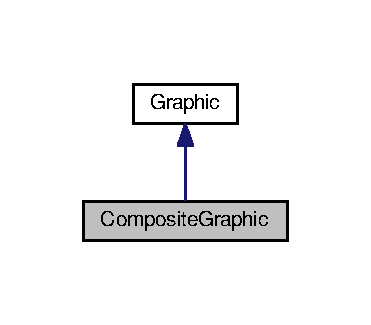
\includegraphics[width=178pt]{classCompositeGraphic__inherit__graph}
\end{center}
\end{figure}


Collaboration diagram for Composite\+Graphic\+:
\nopagebreak
\begin{figure}[H]
\begin{center}
\leavevmode
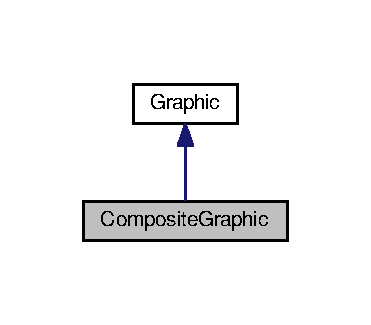
\includegraphics[width=178pt]{classCompositeGraphic__coll__graph}
\end{center}
\end{figure}
\subsection*{Public Member Functions}
\begin{DoxyCompactItemize}
\item 
void \hyperlink{classCompositeGraphic_a0aa29ff6471a74e221c7acf2b2a4cdd4}{print} () const 
\item 
void \hyperlink{classCompositeGraphic_afd74074a4c4429f63585aea1363dd1aa}{add} (\hyperlink{classGraphic}{Graphic} $\ast$a\+Graphic)
\end{DoxyCompactItemize}
\subsection*{Private Attributes}
\begin{DoxyCompactItemize}
\item 
vector$<$ \hyperlink{classGraphic}{Graphic} $\ast$ $>$ \hyperlink{classCompositeGraphic_a3ba19dd348b3579bd2624c964a43422c}{graphic\+List\+\_\+}
\end{DoxyCompactItemize}


\subsection{Member Function Documentation}
\index{Composite\+Graphic@{Composite\+Graphic}!add@{add}}
\index{add@{add}!Composite\+Graphic@{Composite\+Graphic}}
\subsubsection[{\texorpdfstring{add(\+Graphic $\ast$a\+Graphic)}{add(Graphic *aGraphic)}}]{\setlength{\rightskip}{0pt plus 5cm}void Composite\+Graphic\+::add (
\begin{DoxyParamCaption}
\item[{{\bf Graphic} $\ast$}]{a\+Graphic}
\end{DoxyParamCaption}
)\hspace{0.3cm}{\ttfamily [inline]}}\hypertarget{classCompositeGraphic_afd74074a4c4429f63585aea1363dd1aa}{}\label{classCompositeGraphic_afd74074a4c4429f63585aea1363dd1aa}

\begin{DoxyCode}
31                               \{
32     \hyperlink{classCompositeGraphic_a3ba19dd348b3579bd2624c964a43422c}{graphicList\_}.push\_back(aGraphic);
33   \}
\end{DoxyCode}
\index{Composite\+Graphic@{Composite\+Graphic}!print@{print}}
\index{print@{print}!Composite\+Graphic@{Composite\+Graphic}}
\subsubsection[{\texorpdfstring{print() const }{print() const }}]{\setlength{\rightskip}{0pt plus 5cm}void Composite\+Graphic\+::print (
\begin{DoxyParamCaption}
{}
\end{DoxyParamCaption}
) const\hspace{0.3cm}{\ttfamily [inline]}, {\ttfamily [virtual]}}\hypertarget{classCompositeGraphic_a0aa29ff6471a74e221c7acf2b2a4cdd4}{}\label{classCompositeGraphic_a0aa29ff6471a74e221c7acf2b2a4cdd4}


Implements \hyperlink{classGraphic_ab9307ecd30324ec5018ca7d1e88781b9}{Graphic}.


\begin{DoxyCode}
25                      \{
26     \textcolor{keywordflow}{for}(\hyperlink{classGraphic}{Graphic} * a: \hyperlink{classCompositeGraphic_a3ba19dd348b3579bd2624c964a43422c}{graphicList\_}) \{
27       a->print();
28     \}
29   \}
\end{DoxyCode}


\subsection{Member Data Documentation}
\index{Composite\+Graphic@{Composite\+Graphic}!graphic\+List\+\_\+@{graphic\+List\+\_\+}}
\index{graphic\+List\+\_\+@{graphic\+List\+\_\+}!Composite\+Graphic@{Composite\+Graphic}}
\subsubsection[{\texorpdfstring{graphic\+List\+\_\+}{graphicList_}}]{\setlength{\rightskip}{0pt plus 5cm}vector$<${\bf Graphic}$\ast$$>$ Composite\+Graphic\+::graphic\+List\+\_\+\hspace{0.3cm}{\ttfamily [private]}}\hypertarget{classCompositeGraphic_a3ba19dd348b3579bd2624c964a43422c}{}\label{classCompositeGraphic_a3ba19dd348b3579bd2624c964a43422c}


The documentation for this class was generated from the following file\+:\begin{DoxyCompactItemize}
\item 
\hyperlink{Composite_8cpp}{Composite.\+cpp}\end{DoxyCompactItemize}

\hypertarget{classEllipse}{}\section{Ellipse Class Reference}
\label{classEllipse}\index{Ellipse@{Ellipse}}


Inheritance diagram for Ellipse\+:
\nopagebreak
\begin{figure}[H]
\begin{center}
\leavevmode
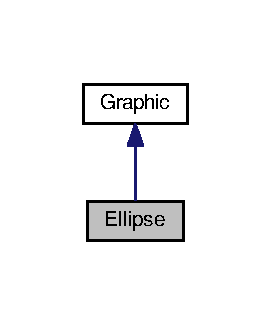
\includegraphics[width=130pt]{classEllipse__inherit__graph}
\end{center}
\end{figure}


Collaboration diagram for Ellipse\+:
\nopagebreak
\begin{figure}[H]
\begin{center}
\leavevmode
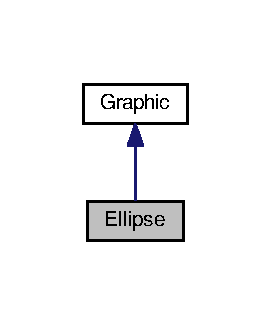
\includegraphics[width=130pt]{classEllipse__coll__graph}
\end{center}
\end{figure}
\subsection*{Public Member Functions}
\begin{DoxyCompactItemize}
\item 
void \hyperlink{classEllipse_a837d8f29455932adf5c639f58f856333}{print} () const 
\end{DoxyCompactItemize}


\subsection{Member Function Documentation}
\index{Ellipse@{Ellipse}!print@{print}}
\index{print@{print}!Ellipse@{Ellipse}}
\subsubsection[{\texorpdfstring{print() const }{print() const }}]{\setlength{\rightskip}{0pt plus 5cm}void Ellipse\+::print (
\begin{DoxyParamCaption}
{}
\end{DoxyParamCaption}
) const\hspace{0.3cm}{\ttfamily [inline]}, {\ttfamily [virtual]}}\hypertarget{classEllipse_a837d8f29455932adf5c639f58f856333}{}\label{classEllipse_a837d8f29455932adf5c639f58f856333}


Implements \hyperlink{classGraphic_ab9307ecd30324ec5018ca7d1e88781b9}{Graphic}.


\begin{DoxyCode}
17                      \{
18     cout << \textcolor{stringliteral}{"Ellipse \(\backslash\)n"};
19   \}
\end{DoxyCode}


The documentation for this class was generated from the following file\+:\begin{DoxyCompactItemize}
\item 
\hyperlink{Composite_8cpp}{Composite.\+cpp}\end{DoxyCompactItemize}

\hypertarget{classGraphic}{}\section{Graphic Class Reference}
\label{classGraphic}\index{Graphic@{Graphic}}


Inheritance diagram for Graphic\+:
\nopagebreak
\begin{figure}[H]
\begin{center}
\leavevmode
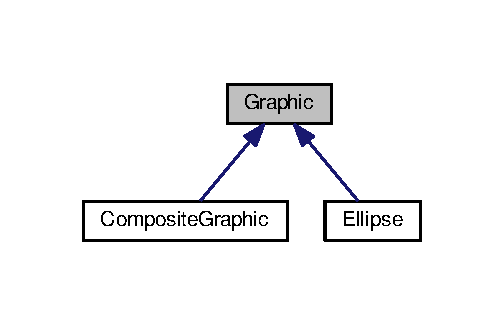
\includegraphics[width=242pt]{classGraphic__inherit__graph}
\end{center}
\end{figure}
\subsection*{Public Member Functions}
\begin{DoxyCompactItemize}
\item 
virtual void \hyperlink{classGraphic_ab9307ecd30324ec5018ca7d1e88781b9}{print} () const =0
\item 
virtual \hyperlink{classGraphic_ab3bbc2327419f52c1e36b626067bf9e1}{$\sim$\+Graphic} ()
\end{DoxyCompactItemize}


\subsection{Constructor \& Destructor Documentation}
\index{Graphic@{Graphic}!````~Graphic@{$\sim$\+Graphic}}
\index{````~Graphic@{$\sim$\+Graphic}!Graphic@{Graphic}}
\subsubsection[{\texorpdfstring{$\sim$\+Graphic()}{~Graphic()}}]{\setlength{\rightskip}{0pt plus 5cm}virtual Graphic\+::$\sim$\+Graphic (
\begin{DoxyParamCaption}
{}
\end{DoxyParamCaption}
)\hspace{0.3cm}{\ttfamily [inline]}, {\ttfamily [virtual]}}\hypertarget{classGraphic_ab3bbc2327419f52c1e36b626067bf9e1}{}\label{classGraphic_ab3bbc2327419f52c1e36b626067bf9e1}

\begin{DoxyCode}
11 \{\}
\end{DoxyCode}


\subsection{Member Function Documentation}
\index{Graphic@{Graphic}!print@{print}}
\index{print@{print}!Graphic@{Graphic}}
\subsubsection[{\texorpdfstring{print() const =0}{print() const =0}}]{\setlength{\rightskip}{0pt plus 5cm}virtual void Graphic\+::print (
\begin{DoxyParamCaption}
{}
\end{DoxyParamCaption}
) const\hspace{0.3cm}{\ttfamily [pure virtual]}}\hypertarget{classGraphic_ab9307ecd30324ec5018ca7d1e88781b9}{}\label{classGraphic_ab9307ecd30324ec5018ca7d1e88781b9}


Implemented in \hyperlink{classCompositeGraphic_a0aa29ff6471a74e221c7acf2b2a4cdd4}{Composite\+Graphic}, and \hyperlink{classEllipse_a837d8f29455932adf5c639f58f856333}{Ellipse}.



The documentation for this class was generated from the following file\+:\begin{DoxyCompactItemize}
\item 
\hyperlink{Composite_8cpp}{Composite.\+cpp}\end{DoxyCompactItemize}

\chapter{File Documentation}
\hypertarget{Composite_8cpp}{}\section{Composite.\+cpp File Reference}
\label{Composite_8cpp}\index{Composite.\+cpp@{Composite.\+cpp}}
{\ttfamily \#include $<$vector$>$}\\*
{\ttfamily \#include $<$iostream$>$}\\*
{\ttfamily \#include $<$memory$>$}\\*
{\ttfamily \#include $<$algorithm$>$}\\*
Include dependency graph for Composite.\+cpp\+:
\nopagebreak
\begin{figure}[H]
\begin{center}
\leavevmode
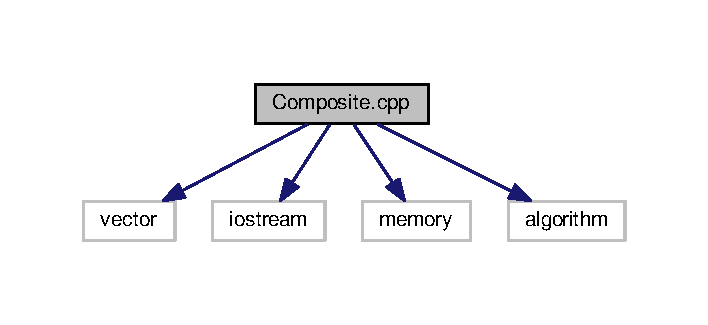
\includegraphics[width=340pt]{Composite_8cpp__incl}
\end{center}
\end{figure}
\subsection*{Classes}
\begin{DoxyCompactItemize}
\item 
class \hyperlink{classGraphic}{Graphic}
\item 
class \hyperlink{classEllipse}{Ellipse}
\item 
class \hyperlink{classCompositeGraphic}{Composite\+Graphic}
\end{DoxyCompactItemize}
\subsection*{Functions}
\begin{DoxyCompactItemize}
\item 
int \hyperlink{Composite_8cpp_ae66f6b31b5ad750f1fe042a706a4e3d4}{main} ()
\end{DoxyCompactItemize}


\subsection{Function Documentation}
\index{Composite.\+cpp@{Composite.\+cpp}!main@{main}}
\index{main@{main}!Composite.\+cpp@{Composite.\+cpp}}
\subsubsection[{\texorpdfstring{main()}{main()}}]{\setlength{\rightskip}{0pt plus 5cm}int main (
\begin{DoxyParamCaption}
{}
\end{DoxyParamCaption}
)}\hypertarget{Composite_8cpp_ae66f6b31b5ad750f1fe042a706a4e3d4}{}\label{Composite_8cpp_ae66f6b31b5ad750f1fe042a706a4e3d4}

\begin{DoxyCode}
40 \{
41   \textcolor{comment}{// Initialize four ellipses}
42   \textcolor{keyword}{const} \hyperlink{classEllipse}{Ellipse}* ellipse1(\textcolor{keyword}{new} \hyperlink{classEllipse}{Ellipse}());
43   \textcolor{keyword}{const} \hyperlink{classEllipse}{Ellipse}* ellipse2(\textcolor{keyword}{new} \hyperlink{classEllipse}{Ellipse}());
44   \textcolor{keyword}{const} \hyperlink{classEllipse}{Ellipse}* ellipse3(\textcolor{keyword}{new} \hyperlink{classEllipse}{Ellipse}());
45   \textcolor{keyword}{const} \hyperlink{classEllipse}{Ellipse}* ellipse4(\textcolor{keyword}{new} \hyperlink{classEllipse}{Ellipse}());
46  
47   \textcolor{comment}{// Initialize three composite graphics}
48   \textcolor{keyword}{const} \hyperlink{classCompositeGraphic}{CompositeGraphic}* graphic(\textcolor{keyword}{new} \hyperlink{classCompositeGraphic}{CompositeGraphic}());
49   \textcolor{keyword}{const} \hyperlink{classCompositeGraphic}{CompositeGraphic}* graphic1(\textcolor{keyword}{new} \hyperlink{classCompositeGraphic}{CompositeGraphic}());
50   \textcolor{keyword}{const} \hyperlink{classCompositeGraphic}{CompositeGraphic}* graphic2(\textcolor{keyword}{new} \hyperlink{classCompositeGraphic}{CompositeGraphic}());
51  
52   \textcolor{comment}{// Composes the graphics}
53   graphic1->add(ellipse1);
54   graphic1->add(ellipse2);
55   graphic1->add(ellipse3);
56  
57   graphic2->add(ellipse4);
58  
59   graphic->add(graphic1);
60   graphic->add(graphic2);
61  
62   \textcolor{comment}{// Prints the complete graphic (four times the string "Ellipse")}
63   graphic->print();
64   \textcolor{keywordflow}{return} 0;
65 \}
\end{DoxyCode}


Here is the call graph for this function\+:
\nopagebreak
\begin{figure}[H]
\begin{center}
\leavevmode
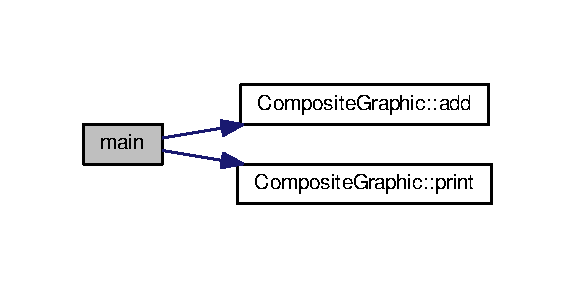
\includegraphics[width=276pt]{Composite_8cpp_ae66f6b31b5ad750f1fe042a706a4e3d4_cgraph}
\end{center}
\end{figure}



%--- End generated contents ---

% Index
\backmatter
\newpage
\phantomsection
\clearemptydoublepage
\addcontentsline{toc}{chapter}{Index}
\printindex

\end{document}
